\subsection{Explicación formal del problema}
Sean $n$ puntos distintos, $(x_1, y_1), \hdots, (x_n, y_n)$, todos pertenecientes al primer cuadrante. Es posible trazar semirrectas de modo que eventualmente todos los puntos estén atravesados por alguna de ellas. La idea es hacerlo de tal forma que cuando se agrega una semirrecta se anota cuántos puntos atravesó y más específicamente cuáles, con la condición de que si un punto es atravesado por 2 o más semirrectas solo se anota para una de ellas. 

En particular, se desea obtener alguna solución óptima para este problema, es decir, una que utilice la mínima cantidad de semirrectas posibles, listando los puntos de la forma antes explicada. 


A continuación, se profundiza la explicación con algunos ejemplos 

\begin{figure}[H]
\centering
\begin{minipage}{0.49\textwidth}
  \centering
    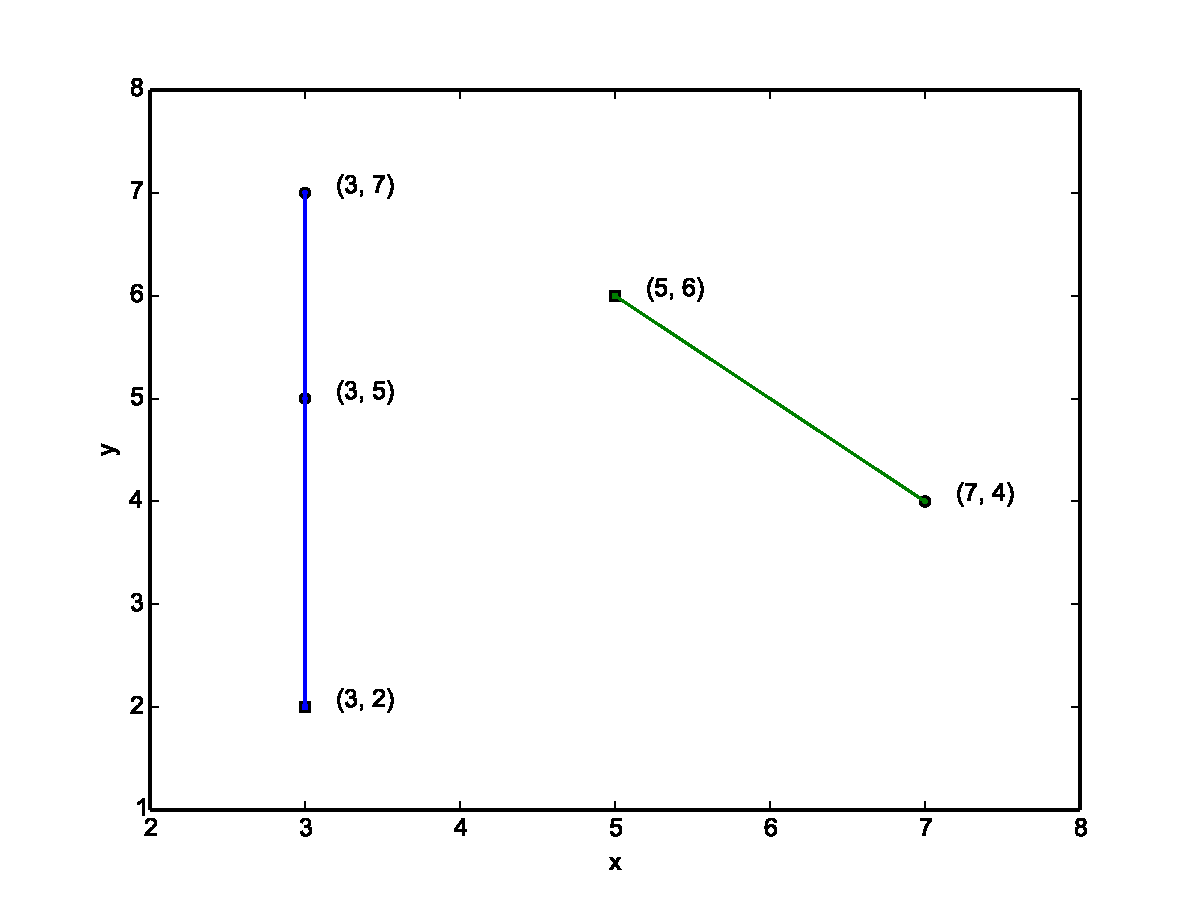
\includegraphics[width=1\textwidth]{img/ejemplos/ej3-1.pdf}
  \caption{\footnotesize Solución óptima para el conjunto dado de 5 puntos, usando 2 semirrectas.}
  \label{fig:ej3-1}
\end{minipage}%
\hspace{0.01\textwidth}
\begin{minipage}{0.49\textwidth}   
  \centering
    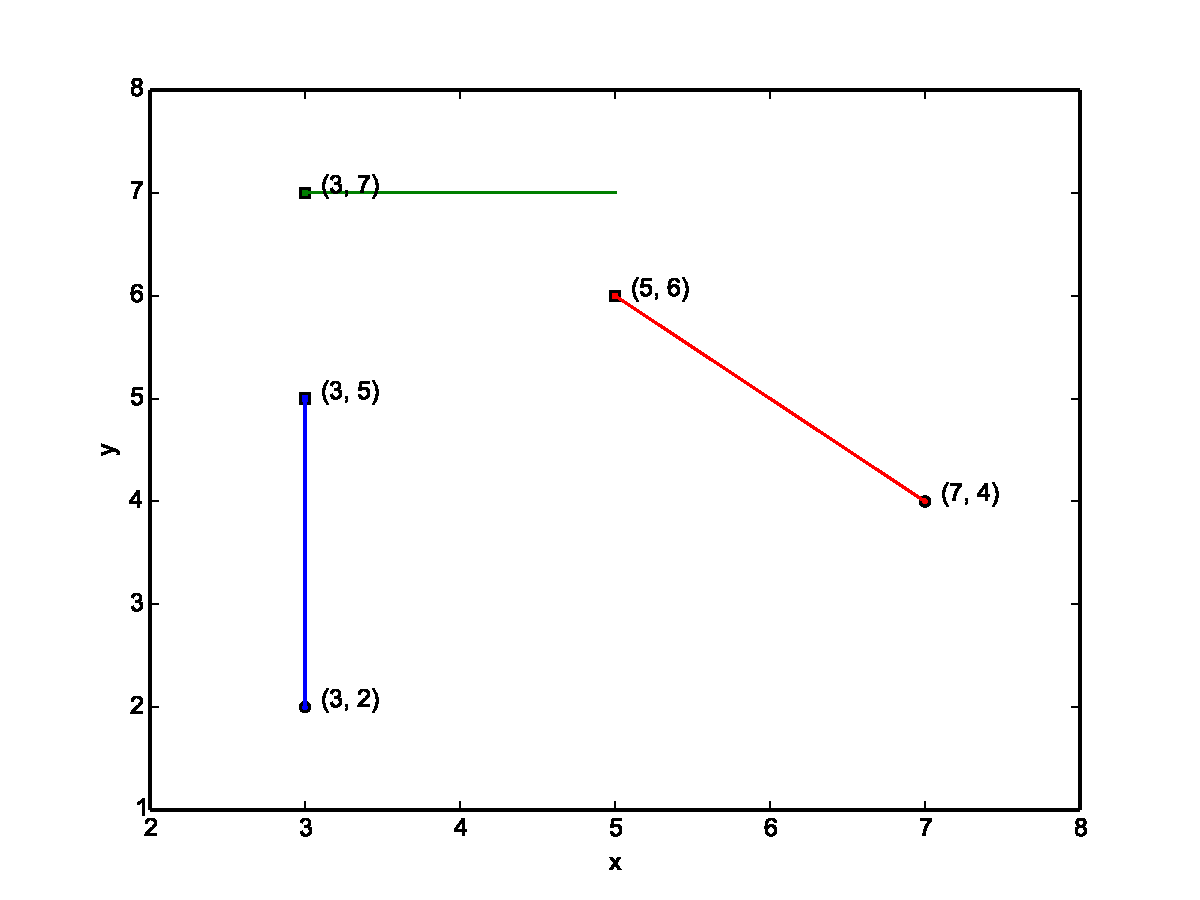
\includegraphics[width=1\textwidth]{img/ejemplos/ej3-2.pdf} 
  \caption{\footnotesize Solución no óptima para el conjunto dado de 5 puntos pues usa 3 semirrectas.}
  \label{fig:ej3-2}
\end{minipage}%
\end{figure}

\begin{figure}[H]
  \centering
  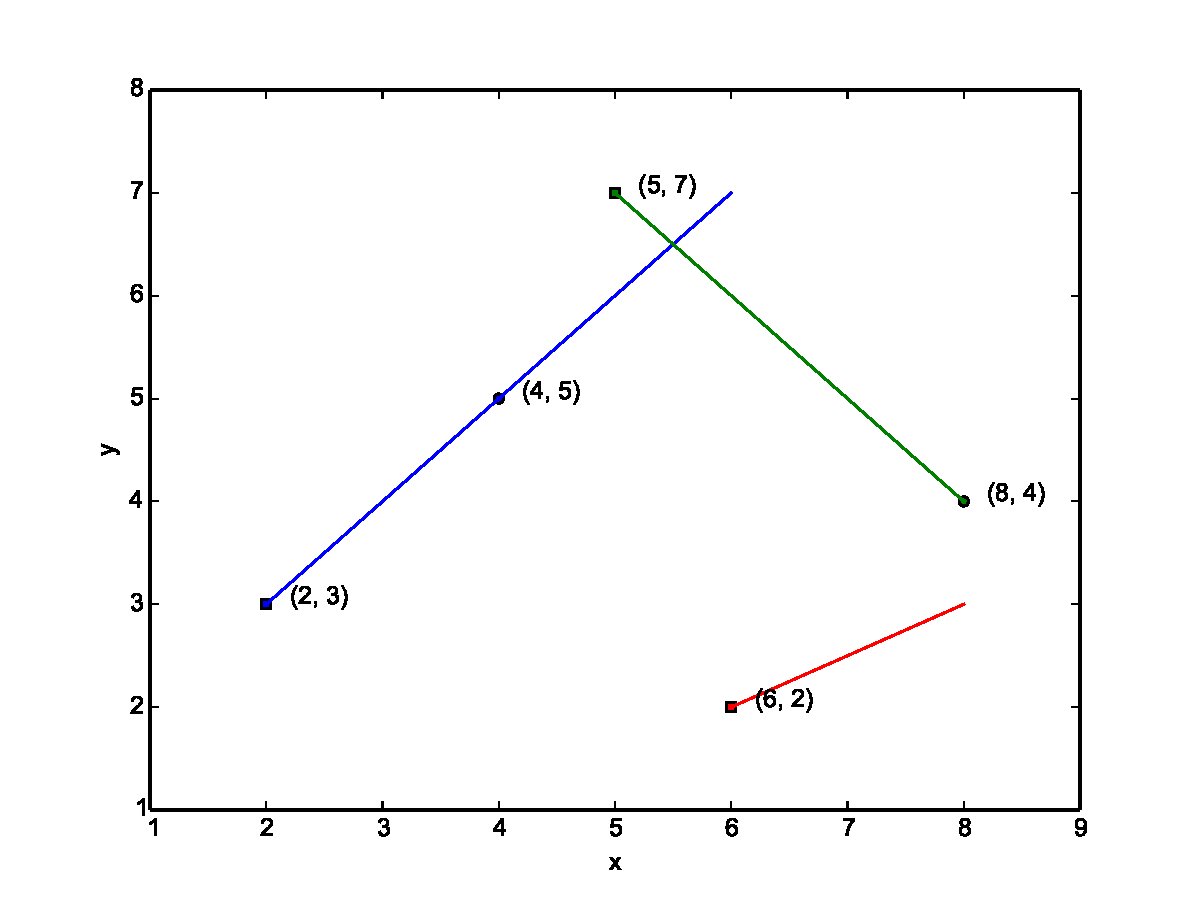
\includegraphics[width=0.75\textwidth]{img/ejemplos/ej3-3.pdf}
  \caption{\footnotesize Solución óptima para un conjunto dado de 5 puntos, donde no hay 3 puntos alineados.}
  \label{fig:ej3-3}
\end{figure}

\begin{figure}[H]
  \centering
  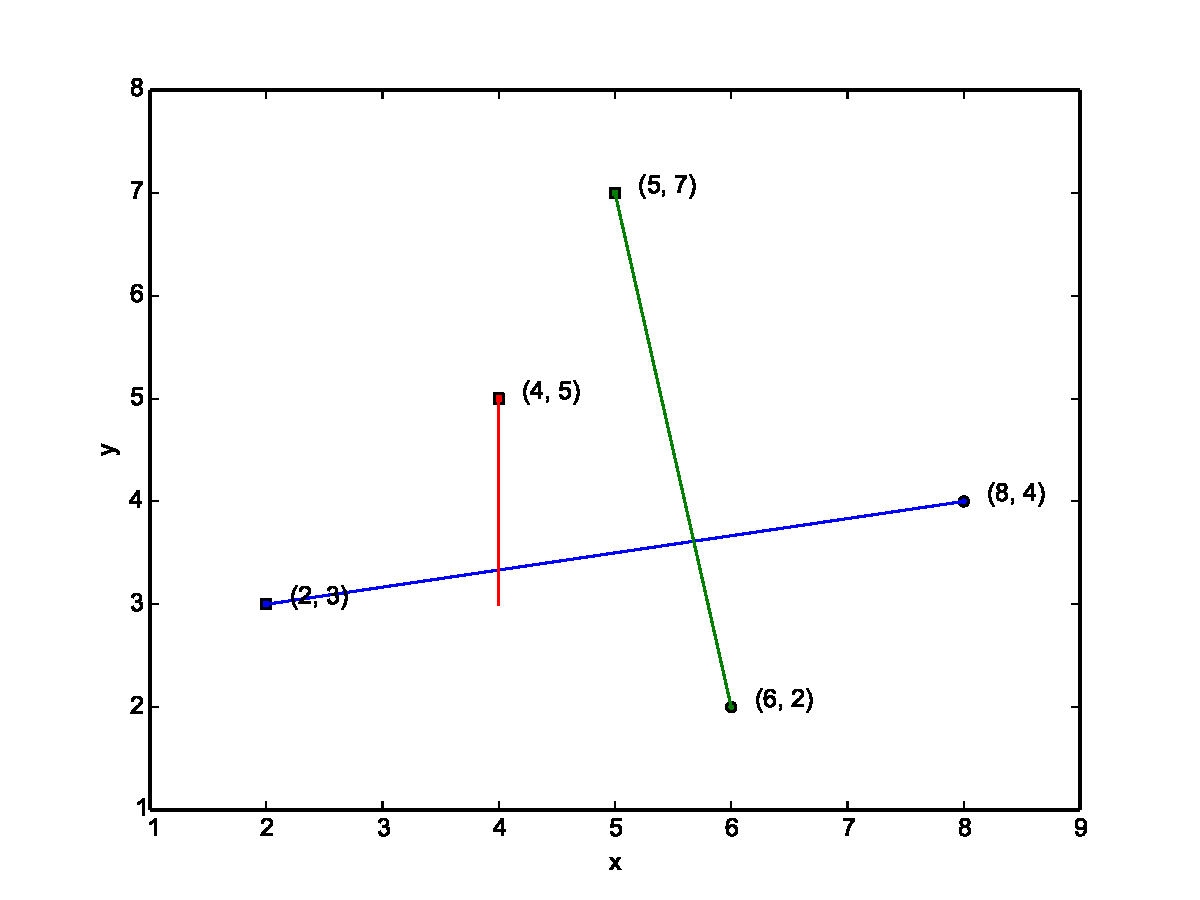
\includegraphics[width=0.75\textwidth]{img/ejemplos/ej3-4.pdf}
  \caption{\footnotesize Solución óptima para un conjunto de 16 puntos dispuestos sobre una circunferencia de radio 2 centrada en $(3,3)$.}
  \label{fig:ej3-4}
\end{figure}

\subsection{Explicación de la solución}
\subsubsection{Árbol de posibilidades}

\subsubsection{Podas}

\subsubsection{Pseudocódigo}
  \begin{algorithm}[H]
  \begin{algorithmic}
  \caption{Pseudocódigo del procedimiento de \texttt{backtracking} en Kamehameha}
    \Procedure{backtracking}{Tablero $t$, int $step$}
    \If {$step \geq mejor$}
      \State $return$
    \EndIf
    \If {$t.Solucionado()$}
      \State $mejor = step$
      \State $mejor\_sol = t.Solucion()$
    \Else
      % \For {$j \in [0,..., n)$}
      %   \If {$j < \frac{n}{2}$}
      %     \State $matrizpeleas[pactual][inicio + j] \gets 1$
      %   \Else 
      %     \State $matrizpeleas[pactual][inicio + j] \gets 2$
      %   \EndIf
      % \EndFor
      % \State $generarpeleas(\frac{n}{2}, pactual+1, inicio)$
      % \State $generarpeleas(\frac{n+1}{2}, pactual+1, n/2 + inicio)$
    \EndIf
    \EndProcedure
  \end{algorithmic}
  \end{algorithm}

\subsection{Complejidad del algoritmo}

\subsection{Performance del algoritmo}